\documentclass[mestrado]{pacotes/unb-cic}
\usepackage[american,brazil]{babel}
\usepackage[T1]{fontenc}
\usepackage{indentfirst}
\usepackage{natbib}
\usepackage{xcolor,graphicx,url}
\usepackage[utf8]{inputenc}
\usepackage{booktabs} % for tables
\usepackage{verbatim} %% multiline comments
\usepackage{dirtytalk} %% Quotes

\graphicspath{ {imagens/} } % path to images

%\bibpunct[; ]{(}{)}{,}{a}{}{;}%muda colchetes para parenteses

% definicoes previas do documento
%\selectlanguage{brazil}
\title{A Run-Time Goal Model for Self-Adaptation in Open-Systems}

\orientador[a]{\prof[a] \dr[a] Genaina Nunes Rodrigues}{CIC/UnB}

\coordenador[a]{\prof[a] \dr[a] Alba Cristina Magalhaes Alves de Melo}{CIC/UnB}

\diamesano{9}{Junho}{2016}


\membrobanca{\prof }{CIC/UnB}

\membrobanca{\prof }{CIC/UnB}

\autor{Gabriel Siqueira}{Rodrigues}

\CDU{004.4}

\palavraschave{dependabilidade}
\keywords{dependability}

%-------------------------------------------------

\begin{document}

\maketitle

\pretextual
%\begin{agradecimentos}
%Agradecemos à nossa orientadora, \prof[a] \dr[a] Genaina Nunes Rodrigues,
%\end{agradecimentos}

%\begin{resumo}
%Nesse trabalho apresentamos...
%\end{resumo}

\selectlanguage{american}

\begin{abstract}%\textbf{}

  In recent years we see a growing availability of devices with computer capabilities. With this come an opportunity for applications that use a number of heterogeneous computer units in an opportunistic way. The development of such application are currently challenging.

  % In a non-adaptive computer systems the computer is static linked to its function in the system.  To achieve a hight level of dependability in such systems one would either rely on right dependable units or on a hight level of redundancy. Both this solutions genearly leads to expensive systems. Appling self-adaptiveness is possible to a system tolerate to failures without a proibit level of redundancy. allow the development of dependable multi-processor heterogeneous systems in face of not dependable units with a lower level of redundancy.

  Our approach is a middleware that permit uses a  multi-agent runtime goal model, in witch agents can accomplish goals by selecting strategies in its local strategies repository, evaluating them by a utility function. On top of this we aim at easy the development of adaptable open-systems applications, allowing runtime discovery of peers and opportunistically sharing tasks between them, easy integration of new functional strategies and easy integration of new adaptation strategies.

\end{abstract}

%\selectlanguage{brazil}
\tableofcontents
\listoffigures
%listoftables

\textual

\chapter{Introduction}
% In the last decade we have seen advances in the study of autonomic computing systems as an alternative to handle the crescent complexity of systems. The complexity in systems come with the need to execute in heterogeneous platforms, to run in multiple environments and handle multiple operation contexts.


With increasing popularity of mobile computation and wireless networks we have seen the rise of  interest in new domains of computation that uses the capacity of heterogeneous computer units in a given location.
Example of such domains are Ubiquitous Computing \cite{bell_yesterdays_2007}, Internet of Things (IoT)\cite{atzori_internet_2010}, Assisted Living\cite{kleinberger_ambient_2007} and Opportunistic Computing\cite{smaldone_improving_2011}. In this domains, the environment has a great level of uncertainty (context variability) as the computational resources greatly varies from place to place.
Solutions for these domains would benefit if they could plan the deployment of the system for a given context. To make this possible the system should handle context variability.

% It's the case of \textit{mobile clouds} witch opportunistically form networks to harvest the power of mobile heterogeneous devices \cite{viswanathan_uncertainty-aware_2015}. Such systems could be mapped to multi-agent systems (MAS). In multi-agent systems each agent is a computerized unit capable of make independent decisions.

Self-Adaptive Systems (SAS) tackle uncertainty by packing together functional code with self-adaptation code capable of handling uncertainty by monitoring the context in order to adapt at runtime.
Architecture-based (or component-based) approaches adapt the systems by acting on components of the system or by replacing them\cite{garlan_software_2009}. A possible solution for development of applications for environment with a high level of uncertainty would be to choose an architecture at runtime for the given environment, distributing software components between available computational units and setting up the right communication channels. But to make it possible we need also a model of the system so we can reason about possible system structure in face of the system requirements and context.
So is important to trace system components back to requirements.

Goal Oriented Requirements Engineering (GORE) approaches have gained special attention as a technique to specify self-adaptative systems. GORE models are design-time models used by system analysts and stakeholders to reason about the system requirements.  Goal modeling represents a shift in relation to Object Oriented approaches as it focus on stakeholder goals and states that the system needs to achieve and not in how it achieves it\cite{ali_goal-based_2010}. Dalpiaz et al.\cite{dalpiaz_runtime_2013} proposed Runtime Goal-Models, for reason about runtime fulfillment of goals.

% DSPL (Dynamic Software Product Lines) provide models to check the configuration of the system.

% why get both together?
 Goal models allow us to reason about the requirements of the system and its execution context. And component based engineering about the system structure. To the best of our knowledge there is no integrated model to reason about the system structure in relation to its contexts and requirements.

% Por exemplo existem contexto em que se faz necessário utilizar diferentes técnicas de tolerancia a falha a depender da criticidade das tarefas e do contexto de execução.
Such model would allow us to built more dependable systems. For example, we could choose to use fault tolerance techniques to more critical tasks of the system.
% desta forma é importante definir perviamente as estratégicas que ele pode atender em tempo de projeto e em tempo de execução garantir que elas sejam implementadas conforme definido em tempo de projeto.

 In this work we will explore the integration of approaches to allow reasoning about the relationship between the system goals, components and context of execution. The objective is be able to create valid deployment configurations, trace the system goals accomplishment at runtime and use fault tolerance techniques to improve the dependability of the system in face of error prone components.

\section{Problem Definition}

% is there any component model suitable to trace goals and component service.

To allow the system make decisions about its structure based on requirements and context we need a model that can correlate this 3 concepts: the system structure, the requirements and the context.

What leads us to or general question:


\setlength{\fboxsep}{10pt}
\noindent\fbox{%
    \parbox{0.95\textwidth}{%
        \textbf{Research Question 1 (RQ1):} What would be a good model of software system that
        could allow for reason about the system structure, context and trace the requirements at runtime? In another words, represent the system requirements, structure, operation context and the relationship between this elements?
    }%
}\bigskip

As this question is too difficult to answer directly we will make a proposal of solution and evaluate it. In this work we choose to represent requirements in a Goal Model based approach, the system structure from an architectural point of view and the context as a data reference resolution process.


\setlength{\fboxsep}{10pt}
\noindent\fbox{%
    \parbox{0.95\textwidth}{%
        \textbf{Research Question 2 (RQ2):} Would a model that represent system requirements at runtime as goals, system organization at a component level and a context as a data reference resolution process a model that satisfy RQ1?
    }%
}\bigskip

Yet in relation to RQ1, to develop what would be a good model we did more questions in relation to the fitness of the model for the purpose of decide on system adaptations. The following is in direction of find if a given configuration of the system is valid.

\setlength{\fboxsep}{10pt}
\noindent\fbox{%
    \parbox{0.95\textwidth}{%
        \textbf{Research Question 3 (RQ3):} How to, using the model from RQ1, verify if systems goals are achievable at runtime in face of deployment (configuration) uncertainty.
    }%
}\bigskip

Beside check the system validity in other to forecast faults we want to be able to tolerate faults. What leads to the next question:

\setlength{\fboxsep}{10pt}
\noindent\fbox{%
    \parbox{0.95\textwidth}{%
        \textbf{Research Question 4 (RQ4):} How to assure that goals are always achieved, if they are achievable, in face of components faults ?
    }%
}\bigskip

This research question is the search to insert fault-tolerance, to achieve dependability of the system in face of not dependable components. To achieve a greater level of manutenability, the faul-tolerance techniques should be portable.


\setlength{\fboxsep}{10pt}
\noindent\fbox{%
    \parbox{0.95\textwidth}{%
        \textbf{Research Question 5 (RQ5):}	Is it feasible to implement fault tolerance techniques (\textit{retry, retry on alternate resource, check-
point/restart and replication}) as portable components that plug in the runtime model of the system?
    }%
}\bigskip

We also want to asses if the model is a practical solution.

\setlength{\fboxsep}{10pt}
\noindent\fbox{%
    \parbox{0.95\textwidth}{%
        \textbf{Research Question 6 (RQ6):} The model could be used to build a middleware that allows systems build on top of it to asses itself capacity of fulfill their requirements, self-heal in case of not and tolerate faults?
    }%
}\bigskip

As a side goal, we want to build a community around the middleware tool so we can evaluate it practical value for development of systems by third party.

\setlength{\fboxsep}{10pt}
\noindent\fbox{%
    \parbox{0.95\textwidth}{%
        \textbf{Research Question 7 (RQ7):} How to engage the scientific community in a common experiment setup for self-adaptation, especially for dependability attributes, so we can compare different approaches ?
    }%
}\bigskip
%
% As it is not enough be possible, it needs to be reproducible:
%
% \setlength{\fboxsep}{10pt}
% \noindent\fbox{%
%     \parbox{0.95\textwidth}{%
%         \textbf{Research Question 8 (RQ8):} Is it feasible to create an integrated development process for self-adaptive software by bridging goal-oriented requirements engineering with architecture-based adaptation?
%     }%
% }\bigskip

\section{Proposed Solution}

This work propose a method for a software centered system to self-configure itself at the level of deployment, driven by a goal model at runtime.
By our approach a device with computing capabilities is able to accept goals, evaluate its capabilities and context and find the software modules that enable it to achieve its goals, fetch and install them.
In response to changes the system can reevaluate its context, capabilities and available software modules and change its deployment.


\section{Contributions Summary}

\begin{enumerate}
\item conceptual model for a component-based runtime goal model
  %\begin{itemize}
  %  \
  %\end{itemize}
\item component-based runtime goal model middleware architecture and development

% \item component-based runtime goal model middleware support for evolvable systems

% \item a model for open-adaptation and opportunistic computing using multi-agent and component-based runtime goal model

\end{enumerate}

\input{intro/plan_for_completion}

\chapter{Background}

%\section{Self-Adaptive Systems}


Self-adaptive systems have been accepted as a promising approach to tackle context change. Self-adaptivesses is an approach in which the system
\textit{"evaluates its own behavior and changes behavior when the evaluation indicates that it is not accomplishing what the software is intended to do, or when better functionality or performance is possible."}\cite{laddaga_self_1997}.

%kramer et al. dream

Self-adaptive software aims to adjust various artifacts or attributes in response to changes in the self and in the context of a software system\cite{salehie_self-adaptive_2009}.

A key concept in self-adaptive systems is the awareness of the system. It has two aspects\cite{salehie_self-adaptive_2009}:
\begin{itemize}
   \item \textit{self-awareness} means a system is aware of its own states and behaviors.
   \item \textit{context-awareness} means that the system is aware of its context,
\end{itemize}

Schilit et al.\cite{klein_survey_2008} define \textit{context} as \say{the sufficiently exact characterization of the situations of a system by means of perceivable information that is relevant for the adaptation of the system}.

Schilit et al.\cite{klein_survey_2008} define \textit{context adaptation} as \say{a system’s capability of gathering information about the domain it shares an interface with, evaluating this information and changing its observable behavior according to the current situation}.


% laddaga1997: it should relies on software informed about its mission and about its construction and behavior.  This implies that the software has multiple ways of accomplishing its purpose, and has enough knowledge of its construction to make effective changes at runtime.

% Such software should include functionality for evaluating its behavior and performance, and the ability to replan and reconfigure its operations in order to improve its operation.  Self adaptive software should also include a set of components for each major function, along with descriptions of the components, so that components of systems can be selected and scheduled at runtime, in response to the evaluators.

% It also requires the ability to impedance match input/output of sequenced components, and the ability to generate some of this code from specifications. In addition, we seek this new basis of adaptation to be applied at runtime, as opposed to development/design time, or as a maintenance activity.


% mape-k

% different approaches ref salehie

% challenges

%
% A self-managed software architecture is one in which components automatically configure their interaction in a way that is compatible with an overall architectural specification and achieves the goals of the system\cite{kramer_self-managed_2007}.

% Component Control
% include the capability to support component creation, deletion and interconnection.

% include facilities to report the current status of components to higher layers and also include the capability to support component creation, deletion and interconnection.
% adjust the operating parameters of components
% self-tuning algorithms, event and status reporting to higher levels and operations to support modification – component addition, deletion and interconnection.
% situation is met that the current configuration of components is not designed to deal with, this layer detects this failure and reports it to higher layers.



% Change Management

% Goal Management

%\chapter{Self-adaptability Architectures}

%\section{Cloud Computing}
%\section{Goal-oriented requirements engineering}

Goal-oriented requirements engineering (GORE) is concerned with the use of goals for eliciting, elaborating, structuring, specifying, analyzing, negotiating, documenting, and modifying requirements\cite{van_lamsweerde_goal-oriented_2001}.

GORE models are the main tool used by system analysts and stakeholders to reason about the system requirements. Goal modeling represents a shift in relation to traditional software development approaches as it focus on stakeholder goals and states that the system needs to achieve and not in how it achieves it\cite{ali_goal-based_2010}. Goal models are graphs representing AND/OR-decomposition of abstract goals down to operationalisable leaf-level goals. \cite{morandini_operational_2009}

A goal is an objective the system under consideration should achieve. \cite{van_lamsweerde_goal-oriented_2001}

\section{TROPOS}
Tropos\cite{bresciani_tropos:_2004} is a methodology for develop multi-agent systems that uses goal models for requirement analyses. Tropos encompasses the software development phases, from Early Requirements to Implementation and Testing.

\subsection{The Tropos key concepts}

The methodology adopts the i* \cite{yu_modelling_1996} modeling framework, which proposes the concepts of actor, goal, task, resource and social dependency to model both the system-to-be and its organizational operating environment\cite{bresciani_tropos:_2004}. In more recent publication \cite{morandini_tropos_2014} about the Tropos modeling framework the concept of \textit{task} was renamed to \textit{plan}.

The following are the key concepts in the Tropos metamodel\cite{morandini_tropos_2014}:

\begin{itemize}
    \item Actor: an entity that has strategic goals and intentionality
    \item Goals: it represents actors’ strategic interests. \texit{Hard goals} are goals that have clear-cut criteria for deciding whether they are satisfied or not. \textit{Softgoals} have no clear-cut criteria and are normally used to describe preferences and quality-of-service demands.

    \item Plan: it represents, at an abstract level, a way of doing something. The execution of a plan can be a means for satisfying a goal or for \textit{satisficing} (i.e. sufficiently satisfying) a softgoal.

    \item Resource: it represents a physical or an informational entity.

    \item Dependency: its a relationship between to actors that specify that one actor (the \textif{depended}) have a dependency to other actor (the \textit{dependee}) to attain some goal, execute some plan or deliver a resource. The object of the dependence is the \texit{dependum}.

    \item Capability: it represents both the \textit{ability} of an actor to perform some action and the \textit{opportunity} of doing this.

\end{itemize}

% TODO Runtime goal models

%\section{Dependability}
Dependability can be defined as the ability of a system to avoid faults in its services
that (1) are more frequent or (2) more severe that is acceptable. Or as the characteristic of a system to be justifiably trusted.

A common terminology used for system deviations as the following: \cite{avizienis_basic_2004}

\begin{itemize}
  \textbf{failure}: or \textif{service failure} is a perceived deviation from the correct service provided by a system.
  \textbf{error}: is a deviation of correct internal system state that can lead to its subsequent failure.
  \textbf{fault}: is the adjudged or
hypothesized cause of an error
\end{itemize}

Dependability include the following attributes:\cite{avizienis_basic_2004}
\begin{itemize}
  \item \textbf{availability}: readiness for correct service.
  \item \textbf{reliability}: continuity of correct service.
  \item \textbf{safety}: absence of catastrophic consequences on the
user(s) and the environment.
  \item \textbf{integrity}: absence of improper system alterations.
  \item \textbf{maintainability}: ability to undergo modifications and repairs.
\end{itemize}


Many means have been developed of how attain the attributes of dependability. This means can be classified as:

\begin{itemize}
  \item \textbf{Fault prevention} means to prevent the occurrence or introduction of faults.
  \item \textbf{Fault tolerance} means to avoid service failures in the presence of faults.
  \item \textbf{Fault removal} means to reduce the number and severity of faults.
  \item \textbf{Fault forecasting} means to estimate the present number, the future incidence, and the likely consequences of faults.
\end{itemize}


% TODO dependability in face of uncertainty

\section{Attain Dependability at Runtime }
To keep dependability in face of uncertainty in the deployment environment some techniques was proposed for runtime analysis at runtime.

Felipe et al\cite{guimaraes_framework_2013} propose a method of fault-tolerance for a scientific workflow execution in grid.

Alessandro Leite \cite{ferreira_leite_user_2014} propose a fault tolerance schema for cloud deployment based on which a fault instance in the cloud is monitored and in case of failure the instance can be restarted or terminated and them a new instance created.

Danilo et al\cite{mendonca_dependability_2015} propose a methodology for fault forecasting by which developer, at design time, annotate the goal decomposition in goal model and specify context variables. A special tool generate a formula for, given a context, evaluate the probability of achieve a goal at runtime.

% Pessoa et al \cite{pessoa_dependable_2015} propose a ... with and evaluate it with focus on safety ...


 % reduce redundancy

%\section{Model Checking}


\chapter{Related Work}
%\section{Self-adaptability}
%\section{Open-Systems}

%\chapter{Model at Runtime}

%\section{Component Based}

Architectural or component-based modes represent the system as

as a gross composition of components, and their properties of interest\cite{garlan_rainbow:_2004}

considerar the system as

%\section{Dependability}
%\input{related/ecs}
\section{Related Work}
\label{related}


Rainbow is a framework for self-adaptation architecture based\cite{garlan_rainbow:_2004}. It keeps an model of the architecture of the system and can be extended with rules to analyses the system behavior at runtime, find adaptation strategies and perform this changes. It separate the functional  code (internal mechanisms) from adaptation code (external mechanism) in a schema called external control, influenced by control theory. \cite{garlan_software_2009}
Different from our proposal Rainbow don't enforce an specific architecture what could be special useful in case of retrofitting a pre-existent systems. Different from our proposal its not goal-oriented an for the best of our knowledge there is no work on how to map goals to  components.

MUSIC project provides a component-based middleware for adaptation that propose to separate the self-adaptation from business logic and delegate adaptation logic to generic middleware. As in our propose it adapts buy evaluate in runtime the utility of alternatives, to chose a feasible one (e.g., the one evaluated as with highest utility)\cite{rouvoy_music:_2009}. As Rainbow, MUSIC is not goal-oriented.
% Yet it provide means of supporting seamless configuration of component frameworks based on local, remote components and services.

Salehie et al. \cite{salehie_towards_2012} propose a run-time goal model and its related
action selection. It models adaptable software as a system that exposes sensors and effectors and  proposes a model consisting in Goals, Attributes and Action for selecting actions that will effect the adaptable software at runtime, giving sensed attributes.
So the adaptation mechanism is to choose the best action given the actual attributes.
As this work it uses explicit runtime goals and make them visible and traceable.
Different from it we use a more symmetric approach that can allow for functional
and adaptation management.
%The validation is make on simulated environment.

Günalp et al. \cite{gunalp_autonomic_2012} propose a middleware for pervarsive software with autonomic capabilities. The approach is service based. It proposes a component written in a custom language and the use of components repository that allows the discovery on new sensors. The system present a support for adaptability by using policies.
% Different from this work it did not present support for collaboration/delegation of goals to another peers. It don't allow for runtime incorporation of adaptation strategies, also.


\section{Conceptual Model}
\label{conceptual_model}

An agent, in multi-agent systems, is an unit in the system capable of take independent actions. In your conceptual model an agent is an independent computational unit that manages its own resources (CPU, memory, disk, sensors, etc).

\begin{figure}
  \centering
  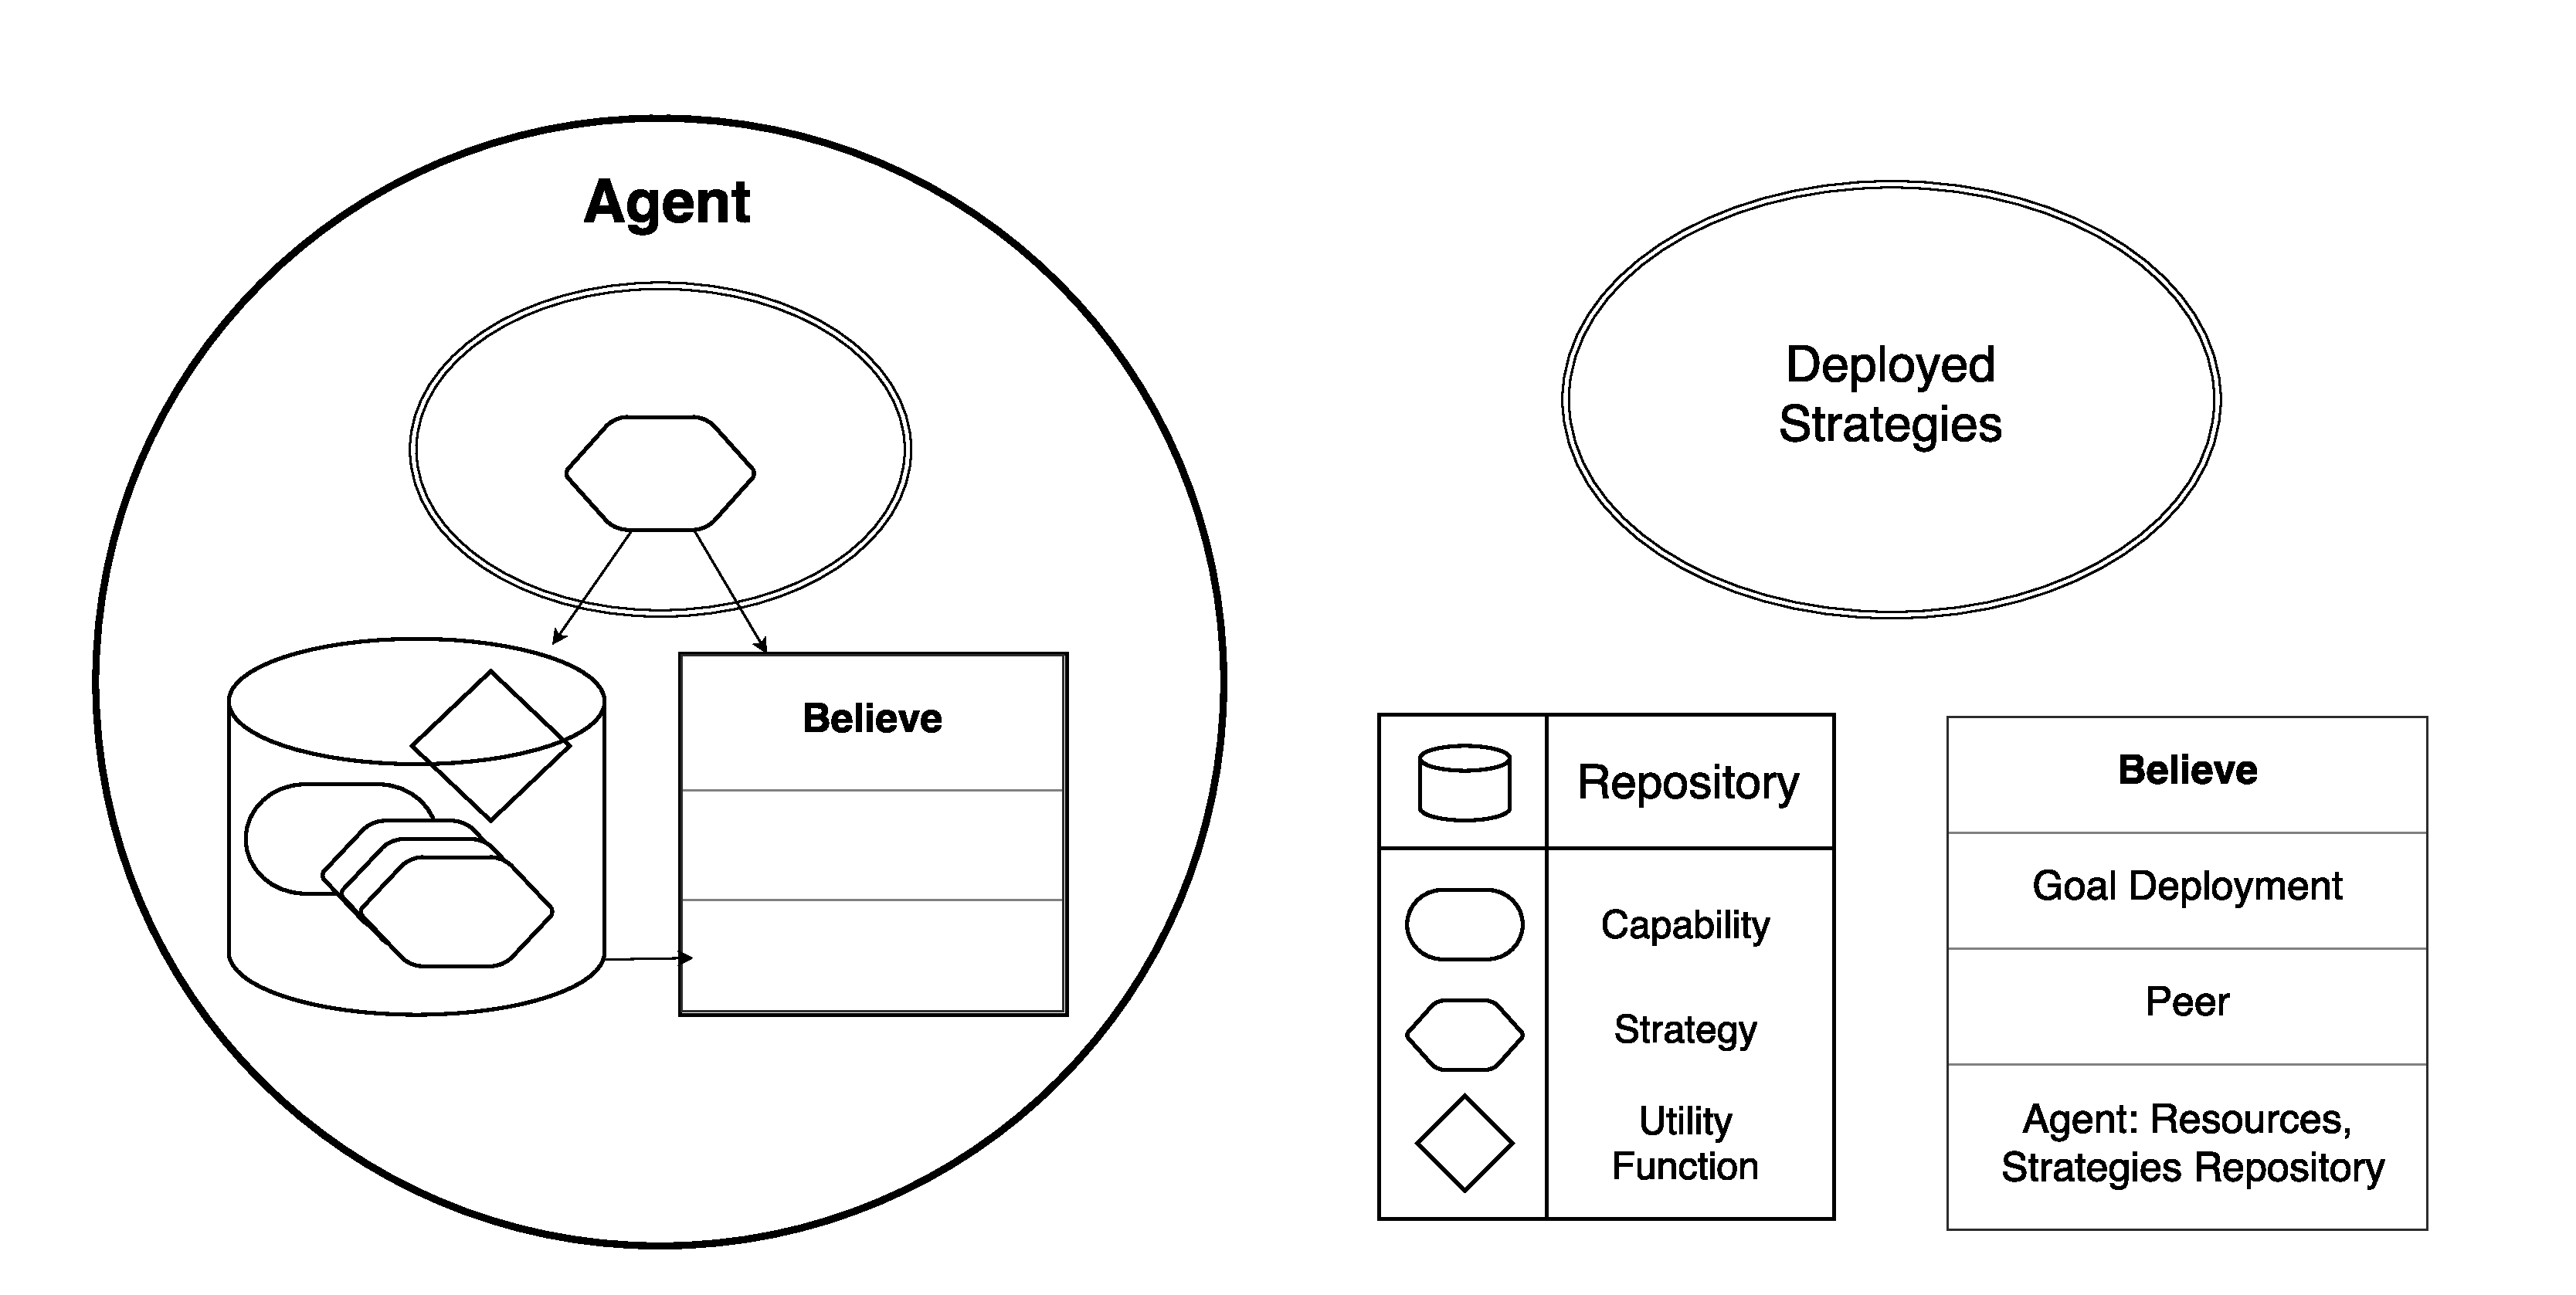
\includegraphics[width=\linewidth]{goalp-agent-repo-rcm-depl}
  \caption{The Agent}
  \label{fig:goalp-agent}
\end{figure}



The system requirements will be represented by 'capacities'. Capacities are what goals a system can accomplish in a goal-model semantics. The system 'capacities' are implemented by 'strategies'.
The 'strategy' is both a mean of achieving a goal (as in GORE) and a component in the architecture. By this we aim at creating an appropriate abstraction to allow composable adaptable architecture while keeping the traceability between the requirements and implementation at runtime.

An agent in the system has a repository of strategies that had all its runnable code. The agent have a model of that repository that it can use for reason about its capacities. The agent can also insert and remove strategies from its repository.

\begin{itemize}
  \item \textbf{Capability}: description of a kind of goal that an agent can perform.   Its an interface description in the architecture. (e.g SUM a and b)
  \item \textbf{Goal Instance}: an actual instance of an objective for a given data set. (e.g SUM 2 and 3)
  \item \textbf{Strategy}: a strategy is a 'Capability Goal' alternative implementation (e.g (SUM,a,b) => {a+b}). Its also a module in the architecture.
  \item \textbf{Strategies Repository}: repository of know strategies
  \item \textbf{Utilitarian Function}: select strategies based on context
  \item \textbf{Runtime Context Model}: data structures that represent the knowledge of the agent.
\end{itemize}

In the proposed model an actor achieve a goal by \emph{deploying a strategy}. For instance the deployment of goals is a capability itself, as follows:

\begin{figure}
  \centering
  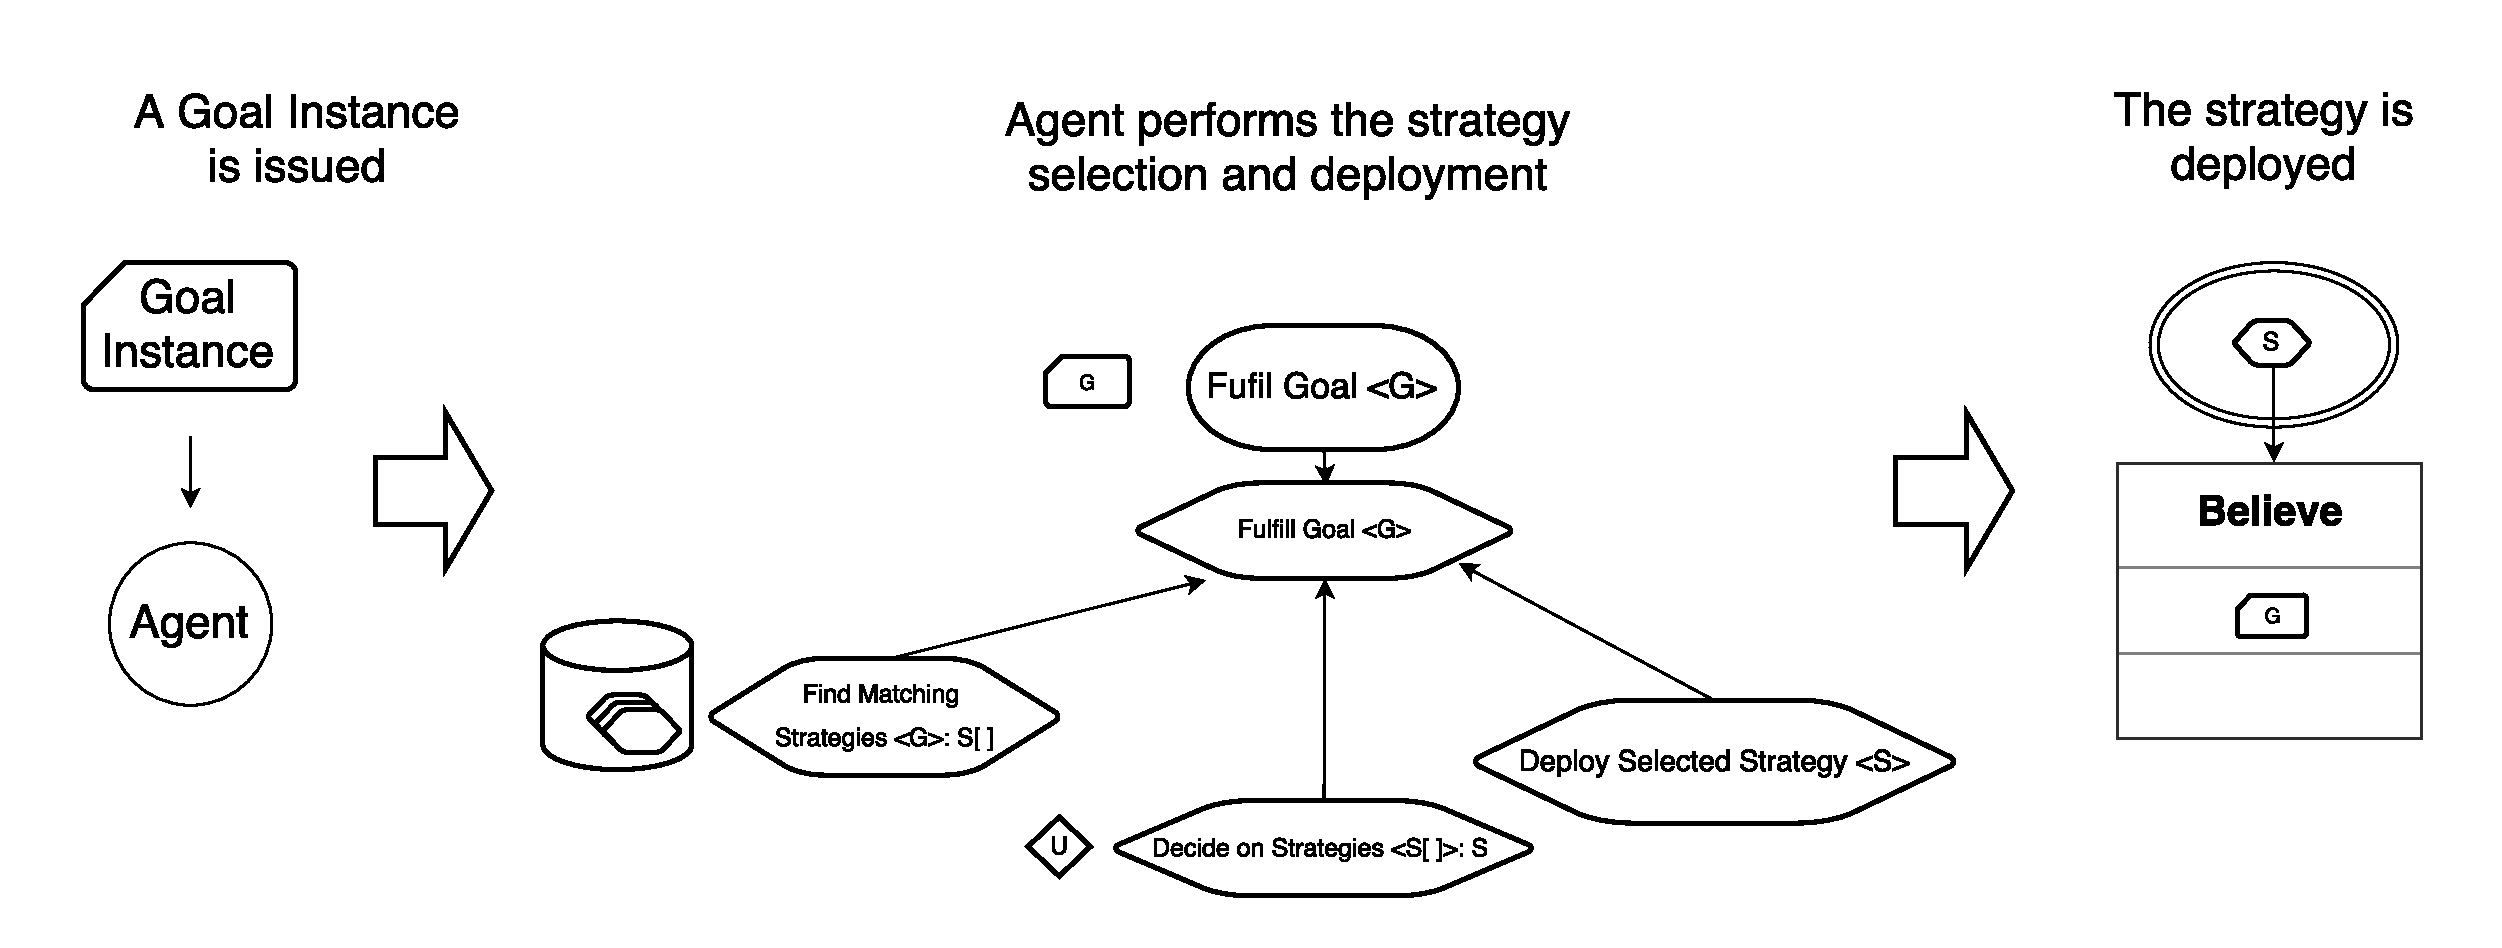
\includegraphics[width=\linewidth]{strategy_deployment}
  \caption{The deployment of a strategy}
  \label{fig:agent_composition}
\end{figure}

\begin{itemize}

\item \textbf{<Fulfill Goals> Goal} the capability of fulfill generic goals.

\item \textbf{<Utilitarianlly Fulfill Goals> Strategy } strategy to fulfill goals by selecting available strategies and evaluating them with an utilitarian function. Consist of 3 sub-goals:
  \begin{itemize}
    \item Find Matching Strategies
    \item Decide on Strategies
    \item Deploy the Selected Strategy
  \end{itemize}
\end{itemize}

And the following three strategies implement the previous 3 goals.

\begin{itemize}
  \item \textbf{<Find Local Matching Strategies> Strategy} accomplish <find matching strategies>
  return the list of matching strategies. An matching strategy is any strategy that implement the goal interface.

  \item \textbf{<Utilitarianlly Select a Strategy> Strategy} accomplish <Utilitarianlly Fulfill Goals>
  use a pre-configured utilitarian function that analyses strategies metadata and select a strategy.

  \item \textbf{<Deploy Strategy> Strategy} accomplish <Deploy Strategy>.
  Consist of call the strategy code for the 'goal issue' runtime context model.
\end{itemize}

%
% \section{Resources}
%
% \section{Strategy Declaration}
%
%
% \section{Fault Model}
% Consistent/Inconsistent Failure
%
% Agent failure
%
% Resource failure
%
% Strategy failure


%\input{content}
%\chapter{Evaluation}
%\section{Evaluation}
%\chapter{Conclusion}
%\section{Conclusion}

\postextual
\anexos


\bibliographystyle{plain}
\bibliography{bibliografia}
\end{document}
